
\chapter{Desenvolvimento da aplicação}
\label{desenv}
Este capítulo apresenta o trabalho desenvolvido numa segunda parte do estágio, o desenvolvimento de um módulo a implementar no produto NkaAcademies. Foi necessário analisar requisitos, tratar da modelação do produto e da sua implementação.

\section{Análise e Especificações}

Na identificação de requisitos são enunciadas todas as funcionalidades, de forma enumerada, que se pretendem implementar no \textit{software}.
Os diferentes requisitos, funcionais e não funcionais, encontram-se classificados pela metodologia \textit{\gls{moscoww}} que identifica os requisitos de elevada prioridade até aos menos prioritários.

Cada tipo de requisito classificado (\textit{\textbf{M}ust}, \textit{\textbf{S}hould}, \textit{\textbf{C}ould}, e \textit{\textbf{W}ould}) representam diferentes significados face ao foco e importância que deverá ser levada em conta durante o processo de desenvolvimento.

Assim sendo:


\begin{enumerate}
  \item \textbf{\textit{Must}}: classificados como requisitos mais críticos ou indispensáveis para o produto, pretende-se o total foco sobre este tipo de requisitos durante o processo de desenvolvimento;
  \item \textbf{\textit{Should}}: são tão importantes como os requisitos classificados como \textit{Must Have}, contudo não são considerados tão priorizados;
  \item \textbf{\textit{Could}}: entende-se como requisitos desejáveis, mas também não são necessários;
  \item \textbf{\textit{Would}}: estes são os requisitos menos críticos e com menor valor, podendo ser implementados ou não.
\end{enumerate}

\subsection{Requisitos Funcionais}

Os requisitos funcionais dizem respeito a todas as funcionalidades ou pressupostos de como o sistema deve reagir a entradas específicas e como se deverá comportar. Estes tipos de requisitos podem-se entender como funcionalidades que o utilizador pode interagir de forma direta e mais visível.

A Tabela~\ref{tab:1} - enuncia os requisitos funcionais estipulados para o sistema.

\begin{longtable}{|l|l|l|l|}

\hline

\textbf{\#} & \textbf{Requisito} & \textbf{Descrição} & \textbf{Prioridade} \\ \hline

RF01 & Pesquisar formação  & \vtop{\hbox{\strut O sistema tem que permitir ao utilizador} \hbox{\strut a procura pelo código da formação ou código} \hbox{\strut de curso}} & MUST \\ \hline
RF02 & Escolher declaração & \vtop{\hbox{\strut O sistema tem que permitir ao utilizador} \hbox{\strut a escolha da declaração que pretende } \hbox{\strut imprimir / preencher.}} & MUST \\ \hline
RF03 & Editar manualmente  & \vtop{\hbox{\strut O sistema deverá permitir ao utilizador a }\hbox{\strut edição manual dos campos a preencher}} & MUST \\ \hline
RF04 & Criar campos  & \vtop{\hbox{\strut O sistema deve permitir a criação de }\hbox{\strut novos campos a serem adicionados às }\hbox{\strut declarações (\textit{template})}} & COULD \\ \hline
RF05 & Editar automaticamente  & \vtop{\hbox{\strut O sistema deverá permitir ao utilizador}\hbox{\strut a edição automática dos campos a preencher,}\hbox{\strut conforme os resultados da procura}}  & MUST \\ \hline
RF06 & Imprimir documento & \vtop{\hbox{\strut O sistema deverá permitir ao utilizador}\hbox{\strut a impressão dos documentos editados.}} & SHOULD \\ \hline


\caption{Requisitos funcionais}\\
\label{tab:1}\\
\end{longtable}

% ------ Req nao Funcionais

\subsection{Requisitos Não Funcionais}

Requisitos não funcionais são as propriedades comportamentais relacionadas ao uso da aplicação em termos de desempenho, usabilidade, confiabilidade, segurança, disponibilidade, manutenção e tecnologias envolvidas. Estes requisitos dizem respeito a como as funcionalidades serão entregues ao utilizador do software.

A Tabela~\ref{tab:2} - encontram-se especificados os requisitos não funcionais do sistema.

\begin{longtable}{|l|l|l|l|}

\hline

\textbf{\#} & \textbf{Descrição} & \textbf{Categoria} & \textbf{Prioridade} \\ \hline

RNF01 & \vtop{\hbox{\strut As novas funções deverão ser implementadas de}\hbox{\strut forma a que sejam compatíveis com outras}\hbox{\strut funcionalidades já existentes}} & Compatibilidade & MUST \\ \hline
RNF02 & \vtop{\hbox{\strut O módulo deverá ser implementado em JavaScript,}\hbox{\strut PHP com acesso à base de dados MySQL}} &  Operacional  & MUST \\ \hline
RNF03 & \vtop{\hbox{\strut Apenas utilizadores autenticados e com permissão}\hbox{\strut devem ter acesso módulo desenvolvido}} & Segurança & MUST \\ \hline

\caption{Requisitos não funcionais}\\
\label{tab:2}\\
\end{longtable}


\section{Arquitetura técnica}

As tecnologias e linguagens utilizadas para o desenvolvimento deste módulo a adicionar ao produto NkaAcademies foram essencialmente descritas no Capítulo~\ref{tecnologias}, com adição de JavaScript e \gls{bootstrap} para desenvolver a componente web da aplicação.

\subsection{Diagrama de Atividades}

Para descrever o processo de negócio foi utilizado o diagrama de atividade, uma vez que permite modelar o comportamento do sistema incluindo a sequência e as condições de execução de ações.

A Figura~\ref{fig:act} demonstra o diagrama de atividades desenvolvido para o sistema.

\begin{center}
        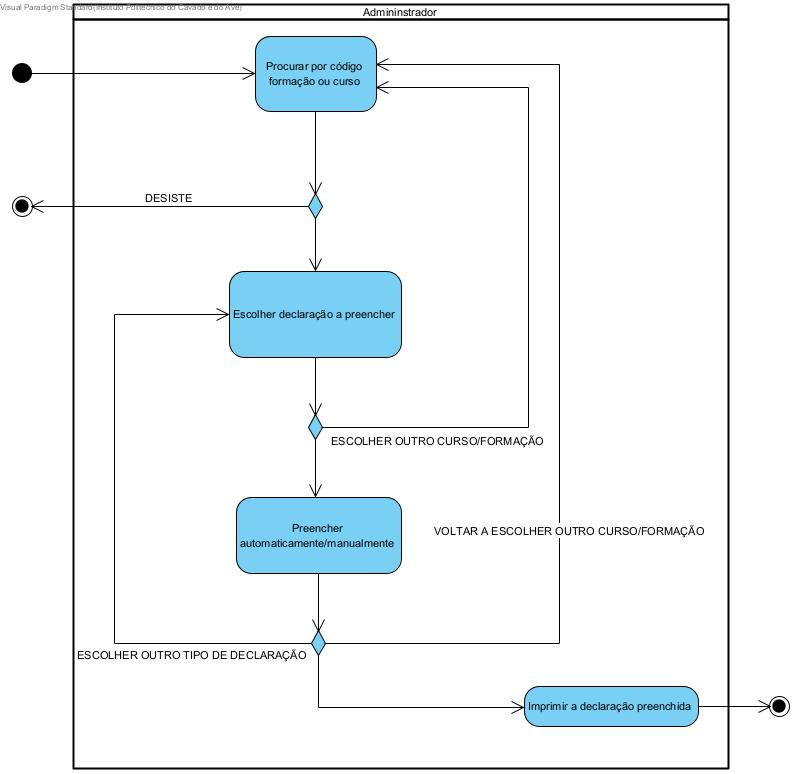
\includegraphics[width=\textwidth,height=\textheight,keepaspectratio]{images/ActivityDiagram1.jpg}
        \captionof{figure}{Diagrama de Atividades}
        \label{fig:act}
\end{center}

Recorrendo à visualização do diagrama da Figura~\ref{fig:act}, é possível perceber os diferentes passos que correspondem à atividade geral do desenvolvimento desta fase do projeto, o preenchimento de documentos de apoio aos processos de gestão de formação. As atividades foram então: filtrar a procura a um resultado, escolher um \textit{template} / declaração predefinido, proceder ao seu preenchimento manual/automático e posteriormente à sua impressão caso seja pretendido.

No desenho deste diagrama está subentendido que o cliente está devidamente autenticado e verificadas as suas permissões no acesso a este tipo de ferramenta dentro da aplicação.

\subsection{Estrutura do código}
% colocar imagem a apresentar a estrutura do código.
Neste sub-capítulo será apresentada a estrutura do código desenvolvido, bem como alguns excertos de código para exemplificar as diferentes camadas existentes no projeto: base de dados, \textit{back-end} e \textit{front-end}.

A Figura~\ref{fig:estrutura} apresenta um esquema gráfico, de forma a que se perceba melhor esta estrutura e as relações entre camadas.

\begin{center}
        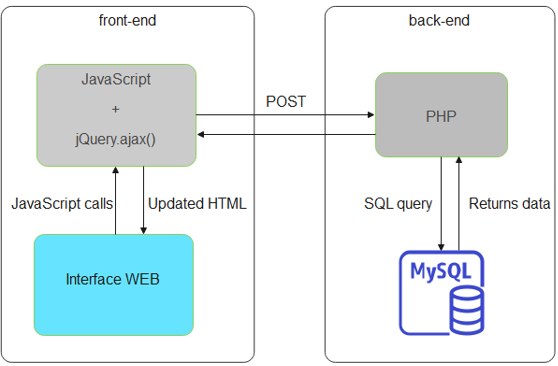
\includegraphics[width=\textwidth,height=\textheight,keepaspectratio]{images/estrutura.png}
        \captionof{figure}{Estrutura do código}
        \label{fig:estrutura}
\end{center}

\subsubsection{Base de Dados}

%A base de dados utilizada para o desenvolvimento deste projeto
Quanto à base de dados utilizada para o desenvolvimento do projeto, não foi feito qualquer tipo de modelação uma vez que foi reaproveitada a base de dados já existente do produto NkaAcademies tendo sido apenas necessário acrescentar alguns dados em tabelas(\textit{templates}) já existentes a fim de testes e futura implementação.

% nao foi feita a modelaçao ao nivel da bd .. apenas foram acrescentadas linhas em algumas colunas (templates) para testes e futura implementação.

\subsubsection{\textit{back-end}}

A parte do \textit{back-end} da aplicação foi desenvolvida em \acrshort{php}. O principal objetivo do trabalho realizado no \textit{back-end} diz respeito a interações com a base de dados, ou seja, tudo que envolva \textit{queries\acrshort{sql}} e ligações a bases de dados são definidas neste sector.

Para uma melhor compreensão, será apresentada na Listagem~\ref{lst:99} um exemplo de uma interação com a base de dados onde basicamente é retornado o conteúdo do \textit{template} selecionado pelo utilizador (\textit{\$\_POST["diploma"]}). Caso se verifique que o \textit{iduser} / cliente existe e o template selecionado está definido na base de dados, é devolvido o seu conteúdo para a interface web.


\begin{lstlisting}[language={php},
                   caption={Exemplo de request à base de dados},
                   label=lst:99]
case 2073:

$result = mysqli_query($con,"SELECT * from xxx.templates
where diploma='".$_POST["diploma"]."'and iduser='$varemp'");

if (mysqli_num_rows($result)!=0)
{
echo str_replace("table table-bordered",
"",utf8_encode(nka_mysqli_result($result,0,"body")));
}
else
{
	echo "Sem Template Definido";
}

mysqli_close($con);

break;
\end{lstlisting}
%-- apresentar como são feitas as interações com a base de dados
\subsubsection{\textit{front-end}}

A parte do \textit{front-end} foi desenvolvida em \acrshort{html}, recorrendo a \textit{modals} do \gls{bootstrap} para implementar a interface web e JavaScript que contém as funções que são o elo de ligação entre a interface web e o \textit{back-end}, que permite atualizar e tornar dinâmica a parte gráfica/visual do sistema.

A Listagem~\ref{lst:98} demonstra a implementação de uma função JavaScript que complementa a ação realizada ao \textit{back-end} na listagem~\ref{lst:99}.

De salientar ainda, a importância do uso de \textit{jQuery.ajax()} que permite utilizar JavaScript para enviar \textit{asynchronous http request} e obter resposta em vários formatos, e também para atualizar partes de uma página web (que use JavaScript) sem ter que recarregar a página web completa \citep{jquery}.

Assim sendo, o \textit{jquery} neste caso é responsável por passar o parâmetro \textbf{diploma} para o \textit{back-end} de forma a ser processada a query\acrshort{sql} correspondente à declaração que o cliente selecionou.



\begin{lstlisting}[language={php},
                   caption={Função JavaScript utilizando jQuery.ajax()},
                   label=lst:98]
function carregatexto(){
    var resultado = $['ajax']({
    type: 'POST',
    url: 'phpScripts/dbload.php',
    data: 'kind=2073&diploma='
        +document.getElementById("template").value,
    async: false })['responseText'];

	$(".summernote").summernote("code", resultado);

	initcampos();
}
\end{lstlisting}


Na Figura~\ref{fig:web} está representada a interface web resultante das listagens de código descritas acima nos pontos \ref{lst:99} e \ref{lst:98}.

De salientar o uso do \textit{summernote} que é uma biblioteca do JavaScript que ajuda na criação de um editor \acrshort{wysiwyg} online \citep{summernote}.


\begin{center}
        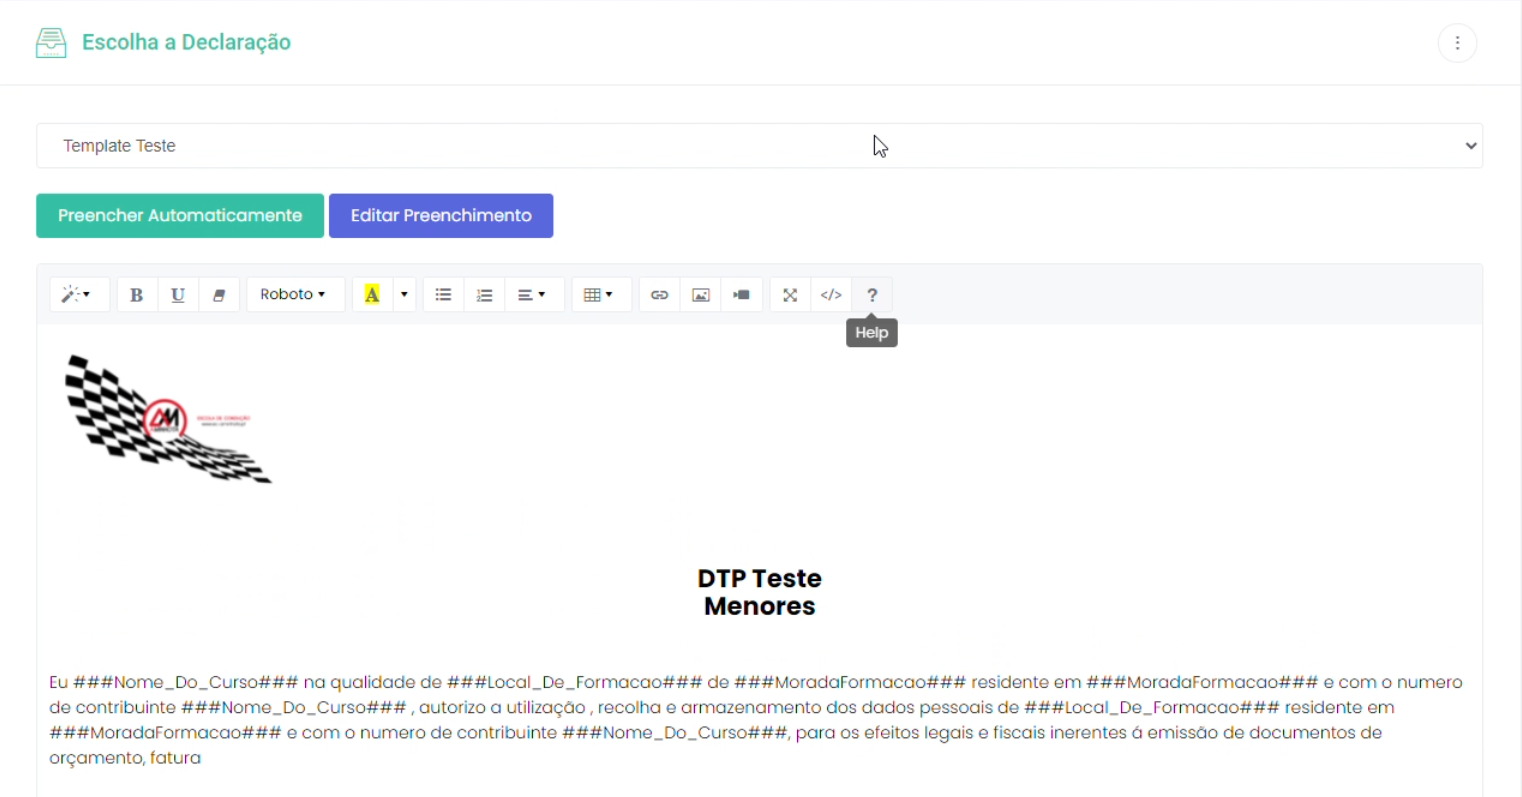
\includegraphics[width=\textwidth,height=\textheight,keepaspectratio]{images/frontend.png}
        \captionof{figure}{Interface Web - template teste}
        \label{fig:web}
\end{center}

% -- apresentar listagem de codigo de como é feito o request ao backend jquery.ajax()
% -- funçoes JS que depois sao chamadas e sao responsaveis por atualizar e tornar responsive a parte da interface web
